\subsection{Data Generation}
\label{sec:soft_cut_data_generation}

The pristine data set contains 1,592 soft cut frames and 637,755 non soft cut frames.
This is a very unbalanced ratio which impedes the training.
To achieve a good generalization of a recurrent neural net, we determined that more data was necessary.
For that, we generated more data by blending random sequences into each other.
A random sequence is picked by reading the gold standard, picking two consecutive elements which encode two cuts with a start and end frame each.
Between the end frame of the first cut and the start frame of the first cut, we can randomly select a subsequence with the desired transition length.
In order to blend two random sequences, we have multiple options for tweening behaviour.
The standard tweening function is linear, but there are also EaseIn, EaseOut etc. (see Figure~\ref{fig:data_generation}).
The tweening function is randomly selected, as well.
As the transition type we used a classic \textit{dissolve}.

In order to achieve further variance in the generated data, we flip the two sequences randomly at the x- or y-axis or at both axes.
With this approach we generated 50 GB of data.


\begin{figure}
    \centering
    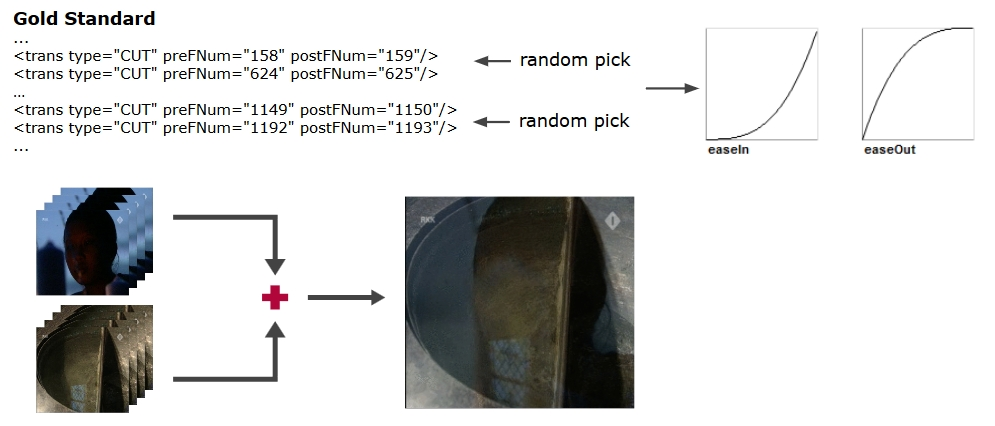
\includegraphics[scale=.5]{images/data_generation.jpg}
    \caption{}
    \label{fig:data_generation}
\end{figure}